\chapter{Related work}

% - 7-22 pages
% - the core element of the thesis, as it shows I'm able to write scientifically.
% - explain what other researchers have found on the topic.
%   - existing approaches (current state of the art, theories, literature (separated by subtopic))
%   - other scientific contributions to solve the task
% - explain the gap in the literature, that the thesis is trying to fill.
%   - new method
%   - new data
%   - new application

%%%%% start writing here

Several tools, frameworks, and even whole ecosystems have evolved around \gls{iacacr}. This chapter is focused on finding the most common, determining their use cases, and identifying their issues.
%TODO only if done: Additionally, a simple reference infrastructure will be introduced, which must be deployable with the respective tool.
%TODO Should the reference infrastructure not be at the top of this chapter? Or at least before the comparison?

\section{State-of-the-art automated hardware provisioning}
The interest in \gls{iacacr} has been increasing on a steady level over the last years \cite{googletrends_iac}. It is estimated that ninety percent of global enterprises will rely on hybrid cloud by 2022 \cite{idc_covid_multicloud}.
Surely boosted by the COVID-19 pandemic, it is also estimated that on-premise workloads drop from 59 percent in 2019 to 38 percent in 2021 and workloads on public clouds grow from 23 percent to 35 percent \cite{thestreet_public_cloud_spending_covid}.
\newline
Instead of updating deployed instances, recreating them ensures all of them are equal \cite{iac_bare_metal}. This includes software and firmware upgrades.
\newline
Another reason is heterogeneity in systems: Even when using only a single vendor or even a single model, variations occur. Be it that newer models have upgraded firmware or other \textquote{under-the-hand} changes \cite{iac_bare_metal}.
\newline
There are differnt opinions on whether a local version of the state should be cached. Some state that it is a necessary means to improve performance \cite{terraform_state}, while others state that it is better not to assume certain states but instead check them \cite{iac_bare_metal}. In case of the latter, whenever a detected state is unexpected, the automation can exclude this certain node and tell the responsible humans to check what's wrong. The most reliable source of truth for the current state is the current state itself - not some kind of cached or partial version of it \cite{iac_bare_metal}.
\newline
So far, public cloud providers haven't exactly published how they are provisioning their bare-metal infrastructure.
\newline
But there are some hints, as some of those providers have an on-premises or edge product. The Microsoft Azure Stack HCI cluster is such a case. The documentation recommends starters to get hardware with the correct drivers and \gls{osacr} preinstalled \cite{microsoft_azure_stack_deployment}. Apart from that, they describe additional \gls{osacr} deployment options like using an answer file (unattended installation), network deployment (\gls{pxeacr}), System Center Virtual Machine Manager (only for Windows \gls{osacr}s), and even manual provisioning \cite{microsoft_azure_stack_deployment}. The preinstalled \gls{osacr} makes the vendor (in this case Microsoft) responsible for provisioning. So it doesn't solve the problem but shifts it somewhere else. Additionally, it doesn't work in all cases - for example on reinstallations.
\newline
While Amazon Web Services Outposts is a similar product, it doesn't allow customers to manage it themselves (and provides no public documentation around it). Instead Amazon dispatch their own service personnel for every necessary manual task \cite{aws_outposts} \cite{aws_outposts_faq}.
\newline
Google doesn't have a product to bring its whole cloud on-premise or to the edge yet, but only dedicated feature sets like the Google Kubernetes Engine. For it, the company relies on an underlying VMware vSphere environment and therefore outsources hardware management \cite{google_anthos_onprem}.
% \newline
% TODO add only when numbers are added below: When a company like Google relies on third-party software it has to be special in some way.

% TODO add VMware numbers here!

So how does the deployment of VMware's vSphere clusters work? The most important thing with the management software called vSphere Server is that it can be deployed as a \gls{vmacr} on an ESXi server (since version 7.0 the appliance is the only way - previously a Windows system could be used as well \cite{vmware_farewell_windows}), the hypervisor \gls{osacr} developed by VMware \cite{vmware_vsphere_installation} \cite{vmware_vcenter_deployment}. In other words, vSphere requires (at least) one manually installed ESXi server, which can then host the vSphere Server software, which then has a feature called Auto Deploy \cite{vmware_installing_esxi}. This feature creates a \gls{pxeacr} boot infrastructure that requires an external DHCP server \cite{vmware_intro_autodeploy} \cite{vmware_autodeploy_process}. The latter has to be configured to distribute network boot details that point to the preexisting vSphere Server \cite{vmware_intro_autodeploy}.
To reduce deployment time, Auto Deploy does not install the ESXi \gls{osacr} on machines but loads the boot image directly into its memory \cite{vmware_provisioning_esxi_using_autodeploy}. This implies that server restarts are handled equally as redeployments.
\newline
Considering VMware develops most of their software themselves (or owns a company that does it for them), the reliance on a third-party product in this field is surprising. But when VMware does rely on this deployment approach, it must have proven to be reliable and hold water. % "stichhaltig"
Apaches CloudStack supports two hypervisors; For ESXi, it recommends also using vSphere, while for XenServer and KVM it does not specify any deployment options - its documentation starts after the hypervisor is installed \cite{cloudstack_installation}.
\newline
One of the most recently published cluster software for bare metal is Google's Anthos. The software and its documentation completely omit the provisioning part up to the point where nodes can only be added when they are already accessible via \gls{sshacr} \cite{anthos_bare_metal}.
\newline
Common asset management tools like servicenow or i-doit use providers like vSphere or public clouds for instantiation \cite{servicenow_setup_guide_vmware_cloud} or even do not support hardware provisioning \cite{idoit_vm_provisioning} at all.
\newline
Other bare-metal lifecycle management tools like Canonical MAAS, Foreman, FOG, FAI, Cobbler, Openstacks Ironic, RackNs Digital Rebar and Equinix Metals Tinkerbell as well as Microsofts System Center Virtual Machine Manager also rely on \gls{pxeacr} for automatic \gls{osacr} deployments \cite{maas_how_it_works} \cite{foreman_what_is} \cite{fog_introduction} \cite{fai_how_does_it_work} \cite{cobbler_documentation} \cite{openstack_ironic_docs} \cite{rackn_what_is_digital_rebar} \cite{tinkerbell_architecture} \cite{microsoft_provision_hyperv_bare_metal}. Most often, they have the required software (the aforementioned \gls{dhcpacr}- and \gls{tftpacr}-server) embedded in some way and only require minor interactions to configure it properly (like setting up the \gls{dhcpacr} range).
\newline
Only the minority of bare-metal provisioning software uses or at least supports \gls{ipmiacr} as tool of the trade. This includes Canonical MAAS (only for power management), OpenStacks Ironic (for power management and reading sensor data), RackNs Digital Rebar and ispsystems DCImanager \cite{maas_snap_power_management} \cite{openstack_ironic_docs} \cite{rackn_what_is_digital_rebar} \cite{ispsystem_dcimanager}.
The main issues with using \gls{ipmiacr} for provisioning are due to is its vendor-specific implementations. Not only is it not available for all hardware, but different vendors support different features (and versions) of \gls{ipmiacr} - often even with different \gls{apiacr}s. A second but closely related issue is its unavailability for \gls{vmacr}s: Most hypervisors don't support \gls{ipmiacr} interfaces for virtual machines. And even if they do (for example via plugins), their documentation is sparse and their development stale \cite{openstack_virtualbmc}.
\newline
Another reason for not using \gls{ipmiacr} is its historically low security. Although most vendors each had their own credentials for accessing the management interface, they used the same combination of user and password for all of their devices \cite{bmc_default_passwords}. Only with senate bill 327 chapter 886 (1798.91.04) taking effect in January 2020, the vendors must now use a unique random password for each machine. Most hardware manufacturers make a huge part of their revenue in the United States or even have their headquarter there. They have since deployed this feature as default for orders worldwide.
\newline
On the other hand, the \gls{bmcacr} has capabilities beyond network boot and \gls{wolacr}. For example, it allows administrators to debug an unresponsive machine, execute hard resets and change \gls{biosacr}/\gls{uefiacr} settings remotely.
So while \gls{ipmiacr} has its place, it is not the go-to technology for automated provisioning.
\newline
Whenever \gls{pxeacr} is used for deployments, as a first step an iPXE image is deployed via \gls{tftpacr}. As described in earlier chapters, iPXE is a very advanced and customizable network boot loader. For one, it is scriptable \cite{ipxe_scripting} - the script can even reside on a network location. Therefore it is very flexible in its configuration during its runtime. And it supports loading the actual \gls{osacr} image via \gls{httpacr} instead of \gls{tftpacr}. Since iPXE is several times smaller and more lightweight than most operating systems, as well as the fact that \gls{httpacr} is significantly more performant than \gls{tftpacr} and there exist better tools around it, this approach does not only speed up the deployment but makes it more reliable and customizable, too \cite{ipxe_uefi_http} \cite{why_ipxe} \cite{foreman_ipxe} \cite{jpmens_network_boot_http}.
\newline\smallskip
The previous part of this chapter focused on the technological \textquote{infrastructure} aspect of \gls{iacacr}. Neither less important, less complex nor less diverse is the \textquote{as code} part.
\newline
As long as few properties change, it is feasible to use command-line arguments to describe the desired state for \gls{iacacr} tools \cite{iac_oreilly}. But with a growing amount of properties the state-space increases, requiring a better way to describe it: Configuration files. The languages used within those files are mostly \gls{dslacr}s.

\section{Domain-Specific Languages for Infrastructure-as-Code}
There is a vast amount of \gls{dslacr}s for \gls{iacacr}. Yet, they greatly differ in their purpose, flexibility, and other parameters. This chapter aims at identifying the differences, comparing them, and finally selecting the most appropriate \gls{dslacr} to be extended to bare-metal.
\newline
Since in most cases there is no obvious perfect solution, the selection process needs first to gather the most prominent options. Because there are many \gls{dslacr}s, languages need to be ruled out based on their limitations afterward. As an intermediate result, two or three languages should remain. These can then be compared on a deeper level, for example, whether their internal design allows it to easily extend it. Based on the better understanding gained in that step, a meaningful decision can be made.

\subsection{Amazon CloudFormation}
CloudFormation supports both \gls{jsonacr} and \gls{yamlacr}, is declarative and typed \cite{aws_cfn_concept}. The typing is done with an additional field \textquote{type} for all components. An example type is \mintinline[bgcolor=lightgray,breaklines]{bash}{AWS::EC2::Instance}, so it has the format of \mintinline[bgcolor=lightgray,breaklines]{bash}{AWS::ProductIdentifier::ResourceType} \cite{aws_cfn_concept}.
\newline
Instead of requiring a command-line tool (there exists one \cite{aws_cf_cli} though), CloudFormation is designed to work by just uploading the file containing the definition. Possible sources are s3-buckets, git-repositories or manual uploads. Redeploys after changes have to be triggered manually. It is implied that the orchestrator is run closed-source by Amazon. Therefore CloudFormation is not only a language by Amazon, but also exclusively for Amazon. Additionally, the user has no (direct) influence on the capabilities of the language and the orchestrator.
\newline
Nevertheless, AWS holds by far the largest market share of the cloud market \cite{statista_marketshare_cloud} and was the first public cloud provider. CloudFormation is, therefore, one of the earliest \gls{dslacr}s for describing infrastructure. It is widely used \cite{stackshare_aws_cloudformation}, and the language itself as well as the tools around it can be assumed to be very mature. There are plugins for most IDEs \cite{github_cfn_lint}. While the open-source linter doesn't guarantee to be all-seeing and perfect, it at least promises to not fail in case it doesn't understand everything \cite{github_cfn_lint}. Under the hood, the linter uses schema validation. Assuming the schema is as mature as the language, it can be reasoned that this guarantees the validity of the definition files. The linter also provides detailed information on what exactly is wrong in such a file as well, making it quite error-prone. There is a so-called \textquote{AWS CloudFormation Designer}, too \cite{aws_cloudformation_designer}. It aims at giving the user a GUI to create his infrastructure definition files.
\newline
As do most languages for \gls{iacacr}, CloudFormation supports custom functions, too. It does so in both \gls{jsonacr} and \gls{yamlacr}. Examples are
\newline % mint doesn't automatically make this linebreak...
\mintinline[bgcolor=lightgray,breaklines]{bash}{{ "Fn::GetAtt" : [ "logicalNameOfResource", "attributeName" ] }} in the former language and \mintinline[bgcolor=lightgray,breaklines]{bash}{Fn::GetAtt: [ logicalNameOfResource, attributeName ]} or the short-version
\newline % mint doesn't automatically make this linebreak...
\mintinline[bgcolor=lightgray,breaklines]{bash}{!GetAtt logicalNameOfResource.attributeName} in the latter.
\newline
Using CloudFormation to describe infrastructure requires a lot of knowledge: Starting from all the products and features AWS has to offer, over different solutions that have (partially) redundant features, up to understanding the AWS jargon. An example for this is \textquote{EC2}: New users have a hard time understanding that \textquote{EC2} is actually a \gls{vmacr} and that there is no \textquote{EC1} or similar.
\newline
Since CloudFormation is limited to AWS, it is incompatible with bare metal. This also means that it can be ruled out for further usage in this thesis. Nevertheless, it is a big player in the league of \gls{dslacr}s, so examining it for reference definitely makes sense (to some extend).

\subsection{OpenStack Heat}
The Heat component from OpenStack is responsible for \gls{iacacr}. It is not a language by itself but supports actually two languages. One is named \gls{hotacr} and the other is Amazon CloudFormation. The former is strongly influenced by CloudFormation \cite{openstack_heat_template_guide}. When the \gls{apiacr} for CloudFormation is used, the Heat component translates the AWS-specific types to OpenStack compatible ones \cite{openstack_heat_architecture}.
\newline
\Gls{hotacr} is designed very similar to its counterpart from Amazon, too: They have the same type system (with different types though) and the same overall structure \cite{openstack_heat_architecture}. The contextual jargon (f.e. \textquote{stack}) is also inspired by CloudFormation.
\newline
Another similarity is the required knowledge about products/components. Sticking to the earlier example of creating a \gls{vmacr}, new users are required to know that the necessary type is \textquote{OS::NOVA::Server}. The \textquote{NOVA}-part comes from the fact that the compute component of OpenStack is named this way.
\newline
There are three ways to communicate with the Heat component; First, the CloudFormation cli-tool. Then an additional commandline tool for \gls{hotacr} \cite{openstack_cli_heat} and an official library in/for python \cite{openstack_python_heat}.
\newline
OpenStack supports bare metal via a component called Ironic \cite{openstack_ironic_architecture}. It is the closest implementation of what this thesis desires to accomplish \cite{redhat_bare_metal}. It supports software-defining how new nodes should be provisioned and implements all necessary features - together with other OpenStack components like neutron for networking, glance for \gls{osacr} images, Keystone for service discovery and Nova for compute node management (f.e. metadata).
%TODO describe later why this doesn't fully satisfy the research question; Bootstrapping is not covered, an OpenStack cluster is required beforehand.

% - OpenStack ironic \url{(https://docs.openstack.org/ironic/latest/user/architecture.html})
%   - installs OS on a local disk
%     -> should the OS be installed on a local disk or does every boot happen via network?
%       -> depends on boot-count and network speed and desired first-boot-time and second-boot-time
%   - verify-HW; verify a node is accessible with HPMI (could be combined with flashing nodes' firmware)
%   - really good overview: https://access.redhat.com/documentation/en-us/red_hat_openstack_platform/15/html/bare_metal_provisioning/sect-introduction

\subsection{HashiCorp Configuration Language and Terraform}
One of the most prominent tools is Terraform by HashiCorp \cite{googletrends_iac}. When it was introduced in 2014, it was primarily focused on \gls{awsacr}, but it evolved a lot since then. Nowadays, Terraform supports far over a thousand providers \cite{terraform_providers}. Of those providers \textquote{only} 160 are aimed at \gls{iacacr} \cite{terraform_providers_infrastructure}. Terraform uses \gls{hclacr} as \gls{dslacr} and is highly plugin-based \cite{terraform} \cite{terraform_docs_extend}. In addition to the custom language, \gls{jsonacr} is supported as well \cite{terraform_syntax}.
\newline
Working with Terraform happens with a command-line executable. The binary loads plugins as needed, communicates with the \gls{apiacr}s of the necessary providers, and gives feedback to the user \cite{terraform_plugins}. To be as efficient as possible, Terraform maintains a local state file \cite{terraform_state}. The file contains the last obtained state of the infrastructure. Since Terraform assumes it is the only component changing the infrastructure, this approach enables it to detect differences locally \cite{terraform_state_purpose}. Afterward, it automatically generates an execution plan on how to eliminate those differences and reach the desired state. The last step is then the execution itself, which is at the same time the only step where communication with external \gls{apiacr}s happens.
\newline
Cross-plugin dependencies are supported by the tool as well \cite{terraform_how_it_works_with_plugins}. This makes Terraform extremely versatile and easily extensible.
\newline
Since the state file is meant to mirror the current state, manual interactions with the infrastructure as well as with the state file are strongly recommended against \cite{terraform_cli_recover}. Another reason is the difficulty of recovering from such state disasters \cite{terraform_cli_recover}.

\subsection{Pulumi}
Pulumi is a relatively new technology. Since its first public release in 2017, it came a long way and now advertises as \textquote{\gls{iacacr} for any cloud with any language} \cite{github_pulumi_first_release} \cite{github_pulumi}. Instead of using \gls{yamlacr}, \gls{jsonacr} or \gls{hclacr}, Pulumi is available as library in several programming languages. Available are these libraries for Node.js, JavaScript, TypeScript, Python, Go(lang), and .NET Core (therefore C\#, F\#, and Visual Basic).
\newline
The very different approach Pulumi takes is extremely interesting: It takes the \textquote{as code} part of \gls{iacacr} to a new level. On the other side, it has no documentation on how to extend it and the current state only supports public clouds and Kubernetes \cite{pulumi_providers}. This renders it basically useless for the scope of this thesis.

\subsection{Open Cloud Computing Interface} % https://occi-wg.org/
Two non-vendor-specific standards for describing \gls{iacacr} in a formal way have emerged. First, \gls{occiacr} which was published by the \gls{ogfacr} in 2011 \cite{occi_core}. Their organizational member list mirrors their mainly academic purpose \cite{ogf_members}. Yet, the website of the \gls{occiacr} standard reveals that the last contribution happened back in 2016, so this project seems to be either abandoned or at least neglected since then.
\newline
\Gls{occiacr} defines a protocol and API for a range of management tasks \cite{occi_about}. Initially designed for \gls{iaasacr}, it has since evolved to serve other models like \gls{paasacr} and \gls{saasacr} \cite{occi_about}. The \gls{ogfacr} is backed by companies such as Dell EMC, NetApp and Oracle \cite{hpcinthecloud_next_ogf} \cite{networkworld_ogf}. Since the launch of the standard, several open-source cloud providers have started to support it, including OpenStack, OpenNebula, and CloudStack \cite{occi_implementations}. The last update of the specification was in 2016 \cite{occi_index}. The IT worlds changes fast, so five years since the last update is a long time.

\subsection{OASIS TOSCA with Simple-Profile}
The second cross-vendor standard that has emerged is called \gls{toscaacr}. It was first published in 2013 by the \gls{oasisacr}. The organisation is well-known for widespread standards like \gls{amqpacr}, \gls{mqttacr}, OpenDocument (used as file format by OpenOffice and LibreOffice), PKCS\#11 (a public-key cryptography standard), \gls{samlacr} (an XML-based Single Sign-On standard and alternative to OpenID Connect), SARIF (standard format for static code analysis results) and VirtIO (the main I/O platform of \gls{kvmacr}) \cite{oasis_standards}. Additionally, its members are not only an overwhelming number of academic or governmental institutions but even more so global players like Cisco, Dell, Google, Huawei, HP, IBM, ISO/IEC, the MIT, SAP and VMware \cite{oasis_tosca_members} \cite{oasis_tosca_obligations} \cite{oasis_members}. The latest contribution was only one week before the time of writing, so its actively pursued and developed \cite{tosca_standard_v2} \cite{tosca_releases}.
\newline
\gls{toscaacr} has been used in some proof-of-concept projects \cite{dsl_for_iac} in 2019, but their results were disappointing: The interfaces between the core standard and the supported providers are described as always out of date, which made even simple operations impossible. The tools of the ecosystem surrounding the standard are said to be non-user-friendly and their learning curves to be flat \cite{adminmagazin_aria_tosca}.
Still, \gls{toscaacr} has a lot of plugins for platforms like OpenStack, VMWare, \gls{awsacr}, \gls{gcpacr} and \gls{azureacr} (obviously strongly related to the earlier mentioned member organizations), configuration management tools like ansible, chef, puppet and saltstack or container orchestrators like docker swarm and kubernetes \cite{opentosca_presentation} \cite{adminmagazin_aria_tosca}, \cite{vmware_tosca_components}.
All those projects conclude that the standard is extremely promising, but the current state makes it impossible to use properly \cite{adminmagazin_aria_tosca}.
\newline
Since then, \gls{toscaacr} 2.0 was released, which introduced huge changes like the transition from XML to the current \gls{yamlacr}-declaration.
\newline
The standard contains the specification of a file archive format called \gls{csaracr}. These archives contain five major parts \cite{opentosca_how_to_csar}:
\begin{itemize}
  \item Type definitions, where properties and interfaces are defined
  \item A topology template, that describes the overall design and how the types should interact.
  \item Deployment artifacts, like images and binaries
  \item Implementation artifacts, like scripts
  \item Management plans that describe certain actions, f.e. how to instantiate a new \gls{vmacr}
\end{itemize}
The original \gls{toscaacr} specification has a strong focus on how things should work together but does neither give complete examples nor describe how applications should be designed. Therefore, in addition to the \gls{toscaacr} standard itself, OASIS also published an extending standard called \textquote{TOSCA Simple Profile} \cite{tosca_simple_profile_v1_3}. While large parts of both specifications are redundant, the Simple Profile provides the types and ecosystem needed for real-world applications of \gls{toscaacr}. Examples are types for Compute, Storage, and Credentials. The reference implementation of the \gls{toscaacr} orchestrator, OpenTOSCA interprets and executes whatever is necessary of a \gls{csaracr} definition is also compatible with the \gls{toscaacr} Simple Profile \cite{opentosca_how_to_csar}.

\subsection{OASIS TOSCA with Cloudify}
Cloudify is another implementation of an \gls{toscaacr} orchestrator, but instead of supporting the Simple Profile, it uses another extension - also named Cloudify. This means that the Cloudify extension provides twin types to the likes of the aforementioned Compute, Storage, and Credentials.
Both \gls{toscaacr} implementations / extensions of the \gls{toscaacr} standard are closely related. even their approach is similar: Both have their orchestrator implemented as the backend of a web application. Both allow visualization and (partial) graphical editing of the \gls{csaracr} definitions. Both provide the user with a catalog of example use cases.
\newline
Cloudify is plugin-based, which allows it to support different providers on different levels and for different areas \cite{cloudify_plugins}. It is very well documented and has many useful integrations like LDAP for authentication and authorization \cite{cloudify_ldap_integration}.

\subsection{Ansible}
Being one of the best-known \gls{iacacr} tools, Ansibles user base is huge and it can be considered very mature. It does support power cycle management and overall \gls{bmcacr} interactions for some hardware providers like Hewlett-Packards remote management software iLO and DELL EMCs counterpart iDRAC \cite{ansible_hpilo} \cite{ansible_idrac}. But for \textquote{general} bare-metal provisioning it mostly relies on external systems like cobbler \cite{ansible_cobbler}.

\subsection{Others}
There are a lot of \gls{dslacr}s around \gls{iacacr}. Many of them were not introduced here. The main reason is that their purpose is different, their approach doesn't fit the use case, or they are too specialized. As an example for the latter, cobbler is only about hardware provisioning, but it is not designed for managing virtual machines or describing applications that run on them. On the other side, VMware vSphere can do most of that (it is not made for describing applications though), but it is primarily GUI based, and therefore only partially usable for \gls{iacacr}.

\section{Exclusion based on limitations}
The tools and \gls{dslacr}s around \gls{iacacr} can mostly be split up into two fields: On one side is the provisioning, where instantiation is the main purpose. On the other side is configuration management, where instantiation is \textquote{assumed} and the goal is to change configurations. Some of the most promiment examples are Terraform, Cloudformation, Heat, and Vagrant for provisioning and Ansible, Chef or Puppet for configuration management \cite{iac_report} \cite{iac_oreilly} \cite{terraform_cloudformation} \cite{terraform_chef_puppet} \cite{atlassian_iac}.
\newline
These two categories are named differently in different sources, for example using \textquote{Infrastructure Definition} as a synonym for provisioning and \textquote{Configuration Registry} for configuration management. Some software like Ansible can also fill both roles \cite{iac_oreilly}.
\newline
The field of configuration management is mainly platform-agnostic. Or more specifically, it does not matter whether it is applying to cloud instances, \gls{vmacr}s or bare-metal. Most of the tools in this area interact with a preexisting \gls{apiacr} for their tasks. This could be the \gls{apiacr} of a cloud provider or \gls{sshacr} access to a \gls{vmacr} or bare-metal machine.
\newline
To bootstrap a whole infrastructure with not preexisting \gls{apiacr}s except for the ones available at a hardware level, this thesis focuses on \gls{dslacr}s that are aimed at provisioning. At the same time, it is relatively easy to create instances (of whatever) by sending requests to a cloud provider or a hypervisor, while doing the same with bare-metal not so much: There is no such \gls{apiacr} - yet.
\newline
As a result, all configuration management \gls{dslacr}s are not eligible. Namely, these are Ansible, Chef, and Puppet (from the introduced languages at least).
\newline
As described earlier, all languages that are imperatively describing infrastructure can be ruled out as well. Funnily enough, this doesn't apply to any of the introduced \gls{dslacr}s for \gls{iacacr}.
\newline
As already stated earlier, Amazon CloudFormation is too AWS-specific to be easily extended to bare-metal and is therefore also not an option.
\newline
The implementations of OCCI-compatible software are severely outdated, and their interrelated deprecation/maintenance levels are confusing to say the least \cite{occi_openstack} \cite{occi_opennebula} \cite{github_tmetsch_occi_os} \cite{github_stackforge_occi_os}.
That, and because the latest release of the OCCI standard was over five years ago, as well as sources stating OCCI software does not work even with basic examples, together with an accompanying recommendation to use \gls{toscaacr} instead \cite{dsl_for_iac}, OCCI will not be looked at in too much detail as well. For example, the documentation for the OpenStack implementation \cite{occi_openstack} recommends to visit the corresponding wiki-site, which is even older \cite{openstack_occi}.
\newline
Due to its origin, OpenStack Heat definitely has the ability to possibly solve the initially described problems of this thesis. Sadly enough, its documentation leaves much to be desired \cite{openstack_heat}. Additionally, there are few examples, and to run it even in a proof-of-concept style requires installing and running many components of OpenStack. These requirements make it not only unfeasible for smaller infrastructures, but for "from-scratch" deployments like the one desired in this thesis as well.
\newline
While Pulumi has an extremely interesting approach with using actual programming languages as a medium, it is neither easily extensible nor does it aim at provisioning infrastructure itself. Instead, it parses the infrastructure code and communicates with the corresponding providers. Based on both of these limitations Pulumi is not a valid potential candidate for the scope of this thesis.
\newline
\Gls{toscaacr} has several implementations and corresponding (inofficial) extensions like Cloudify, Alien 4 Cloud, or Puccini. It is out of this thesis' capabilities to compare all of them. Therefore, only the official extension, named \textquote{Simple-Profile} will be included in the comparison.

\begin{table}[H]
  \caption{Overview of language candidates that are ruled out}
  \begin{tabular}{ | l | l | }
    \hline
    Language & Reason \\
    \hline \hline
    Ansible, Chef, Puppet & \makecell{Ruled out because they are made for configuration \\ management, not provisioning.} \\
    \hline
    CloudFormation & Ruled out because it is too AWS-specific. \\
    \hline
    OCCI & \makecell{Ruled out because of old/outdated specificiation \\ and tools.} \\
    \hline
    Heat/HOT & Ruled out because of unfeasable prerequisites. \\
    \hline
    Pulumi & Ruled out because only public clouds and kubernetes are supported. \\
    \hline
    inofficial TOSCA extensions & \makecell{Ruled out because too many and closely related to \\ original TOSCA.} \\
    \hline
  \end{tabular}
  \label{tab:afterculling}
\end{table}

\section{Dimensions of a comparison}
Choosing and selecting the best language for a task is hard. Not only is it hard to agree on what is important to compare, nor is it just time-consuming, but it is greatly domain-specific as well.
There exist multiple comparisons or -methods for \gls{dslacr}s already, most of which are not infrastructure-specific \cite{comparative_study_of_dsl_tools} \cite{comparing_gpl_dsl} \cite{dsl_for_iac} \cite{allgemeine_modeltheorie}.
They compare based on attributes like (no specific order):

\begin{itemize}
  \item Primary approach \cite{comparative_study_of_dsl_tools}
  % \item Abstraction level: don't describe all attributes, but only the relevant ones \\cite{comparing_gpl_dsl} % TODO add mode lecture notes as source
  % \item Isomorphism: Statements for the modeled entities hold for the real world \\cite{comparing_gpl_dsl} % TODO add mode lecture notes as source
  \item Guarantees provided in case of well-formedness \cite{comparative_study_of_dsl_tools} %TODO this also contains "efficiency" like parallelism
  \item Reusability of components \cite{comparative_study_of_dsl_tools}
  \item Error proneness and reporting like line number and column offset \cite{comparative_study_of_dsl_tools} \cite{comparing_gpl_dsl}
  \item Efficiency: Amount of code for a given case study \cite{comparative_study_of_dsl_tools}
  \item Aspects to learn for a given case study or how hard the mental operations are \cite{comparative_study_of_dsl_tools} % / learning-curve
  \item Viscosity: How hard it is to make changes/updates \cite{comparing_gpl_dsl}
  \item Hidden dependencies like requiring agents, a dedicated server or a third-party software \cite{comparing_gpl_dsl}
  \item Visibility: How easy is it to find the responsible snippet in the codebase \cite{comparing_gpl_dsl}
  \item Extensibility: Can the language be adapted to environment changes
  \item Maturity (documentation, user-base, community): How good are edge-cases documented and how well is the product established
  \item Ecosystem
  % Maybe costs as well?
\end{itemize}

The landscape of infrastructure is ever-changing - and so are the used tools and protocols. Therefore, \textquote{extensibility} is another property this thesis is going to consider.
\newline
Also, younger products tend to change a lot at the beginning, while older products have a hard time coping with change. Because of that, another property that is going to be compared is the \textquote{maturity}. It also relates to the covered edge cases which take into consideration the size of the user-base and the quality and quantity of the documentation.
\newline
Very important for the \gls{dslacr} in this thesis is the \textquote{ecosystem} surrounding it. This aims at the software that interprets the language, derives actions from it, and executes them.
\newline
Some of the chosen sources describe more dimensions for their comparisons. While these are useful in general, it was either clear that all languages would perform the same or they are specifically hard to measure (objectively or in a reasonable amount of time). %TODO might add examples here.
\newline
It is important to note that it is out of this thesis' scope to compare the languages on a deeper level, for example, their abstract syntax (i.e. meta models) or their (Extended) Backus-Naur forms. While the selection process is an important part, the goal of this thesis is not to find the perfect \gls{dslacr} but to find a fitting one and extend it so it can be applied on bare-metal.

% what to compare:
% http://www.cse.chalmers.se/~bergert/slides/guest\_lecture\_DSLs.pdf
% - abstract syntax: meta-model which defines parts/domain-concepts/model-elements and rules/validation of model
% - concrete syntax: representation of model (instances) f.e. in an editor
% - static semantics: evaluatable without executing/interpreting the model
% - dynamic semantics: what the model means or expresses

\section{Comparison}
Previously, many \gls{dslacr}s were ruled out, so this thesis is going to look at the remaining three languages in more detail. These are HashiCorp Configuration Language (HCL) with the tool Terraform and TOSCA in combination with its \textquote{Simple-Profile} extension.

\subsection{HashiCorp Configuration Language and Terraform}
The Configuration Language used by Terraform is a mixture between \gls{jsonacr}, \gls{yamlacr} and a programming language like Golang.
To give a first impression, the \gls{jsonacr} in code-snippet \ref{code:json_example} expresses the very same as the \gls{hclacr} in code-snippet \ref{code:hcl_example}.

\begin{listing}[H]\begin{addmargin}[2em]{2em}\begin{minted}[linenos,bgcolor=lightgray,breaklines,escapeinside=||]{json}
  "resource": {
    "aws_instance": {
      "example": {
        "instance_type": "t2.micro",
        "ami": "ami-abc123"
      }
    }
  }
  \end{minted}
  \caption{\gls{jsonacr} example}
  \label{code:json_example}
  \end{addmargin}
\end{listing}

\begin{listing}[H]\begin{addmargin}[2em]{2em}\begin{minted}[linenos,bgcolor=lightgray,breaklines,escapeinside=||]{bash}
  resource "aws_instance" "example" {
    instance_type = "t2.micro"
    ami = "ami-abc123"
  }
  \end{minted}
  \caption{\gls{hclacr} example}
  \label{code:hcl_example}
  \end{addmargin}
\end{listing}

The language can display the same amount of information more densely. This has both positive and negative effects: On one hand, the fewer brackets enable users to focus on the actual content. On the other hand, it is a language on its own, and developers first need to learn it.
\newline
The architecture of Terraform is highly plugin-based and these plugins are often developed by third parties. Terraform accomplishes its integration with those via \gls{rpcacr}. This means, that each plugin is an executable on its own. And when deploying with Terraform, it simply invokes the necessary executables. When invoked, plugins could use a library dedicated for the provider, communicate with \gls{apiacr}s or invoke other executables. This approach also allows plugin developers to decide on the programming language of their choice. At the same time, it outsources authentication for each provider to the corresponding plugin. The core Terraform executable detects necessary plugins out of the provided code and downloads them automatically from a repository like the Terraform registry.
\newline
Still, the plugin system is a curse and blessing at the same time. It enables extraordinary extensibility, yet makes it hard to reuse snippets - what works for one provider most often doesn't work for another that provides the very same feature set. On the other side, being able to share the same provider integration across organizations is a huge bonus that reduces overall duplicate work. The system allows for cross-plugin dependencies so that every infrastructure integration can be described. But the quality of the ecosystem depends on the quality of the plugins in most cases. Since Terraform's user base is huge, most plugins are relatively mature. This means most edge cases are covered, the documentation is great, and most features of a provider are available.
\newline
In larger environments, making the correct change to the infrastructure described with \gls{hclacr} can be hard. Not only does the developer need to know all used technologies, platforms, providers, and their specific products and jargon used in the state description, but it has to determine which one relates to the bit it wants to change as well. For example, some providers only have to provide \gls{vmacr}s, while others provide managed clusters of specific software (databases, Kubernetes, ...).
\newline
Using Terraform comes with three steps: Authoring the infrastructure configuration as code, (automated) planning on how to achieve the desired state, and applying/provisioning the desired infrastructure \cite{terraform_workflow}. The authoring part is self-explaining. The planning is done automatically by the Terraform executable \cite{terraform_workflow}. It compares the state described in the code with the current state and creates an execution plan, where things are parallelized as much as possible.
\newline
Instead of retrieving the current state via \gls{apiacr}s directly from the providers, Terraform maintains a local state(-file). Apart from mapping configuration to real-world instance identifiers (like an \gls{vmacr}-identifier) it is used to significantly improve the performance of the planning phase \cite{terraform_state}; The local mirroring of the actual state enables Terraform to work with the state as fast as a local file-access instead of requiring several \gls{apiacr}-requests. This is especially convenient in large environments, where the provisioned state consists of hundreds or thousands of instances \cite{terraform_state_purpose}.
The local caching of the state has the downside that it is required to sync the state of all invocations of Terraform for the same infrastructure \cite{terraform_state_purpose} in order to prevent race conditions when deploying. If Terraform is integrated into a sole \gls{cicdacr} pipeline this is not a problem as there is only one instance. For all other cases, the documentation of Terraform recommends using a so-called remote state backend that provides state locking as the main feature \cite{terraform_remote_state}. Supported backends range from a shared folder over Terraform Cloud to S3-compatible object storage.
\newline
It is strongly advised against manipulating the state manually \cite{terraform_state}. Errors are hard to debug since Terraform assumes that the state is always valid. Apart from manual changes, failures during state migration (when applying a new state and writing it back to the state file) can result in almost unrecoverable crashes of Terraform \cite{terraform_no_rollback}.
\newline
At the same time, it is strongly advised against manual changes in the infrastructure without using Terraform to get there. After such changes, Terraform might be unable to find that component later and assumes it doesn't exist.

% Terraform:
%   structure:
%     - main.tf ; contains:
%       - terraform configuration/settings (provider, f.e. aws-cli)
%       - provider-specific configuration like region, profile
%       - resources -> 'resource "<type>" "<name>" {...}' -> id == <type>.<name>
%     - variables.tf ; contains
%       - input variables (typed, via param), used with 'var.<variablename>'
%     - outputs.tf ; contains which values should be output when apply is ran
%   validation/error-reporting:
%     - `terraform fmt`: format configuration
%     - `terraform validate`: validate configuration
%   visibility:
%     - all *.tf files are considered and read, so it is possible to split as much as you want - in the same directory
%     - components in subfolders should be made tf-modules
%       - at least one module; called root-module in the main dir
%       - modules can be called multiple times
%       - modules can have input variables, which can be passed from the caller (used with 'module.<modulealias>.<variabelname>')
%       - modules are defined by source-uri, which might be a relative dir-path, http, git, registry, s3-bucket ...
%     - visibility depends on module-structure
%   viscosity:
%     - updates in all directions seem to be quite easy or at least the tooling is there - for debugging as well
%   consistency:
%     - providers and modules are developed by different people, so they tend to be inconsistent.
%     - overall structure is predefined
%   notes:
%     - purpose of the statefile:
%       - how should terraform know to delete a resource (and dependencies and their destruction order) when its not in the config file any more?
%       - for larger infrastructure, querying everything for each action is too much overhead and might become a problem with rate limits
%       - local state contains plain initial passwords, remote state might be encrypted
%       - only tf-internal use recommended, use json flag for output commands
%     - multiple environments/workspaces sometimes supported; dev, prod, local etc.
%     - wants every external file to be translated to own file-format, f.e. dockerfile \url{https://learn.hashicorp.com/tutorials/terraform/docker-build?in=terraform/docker-get-started}

\subsection{OASIS TOSCA with Simple-Profile}
As described earlier, in \gls{toscaacr} infrastructure is modelled via \gls{csaracr} files. As described in figure \ref{image:tosca_overview}, these archives contain multiple parts. These can be defined in one or multiple \gls{yamlacr} files. The main component is the so-called Topology Template. It describes how the different parts of a system interact with each other, gives a holistic overview, and defines variable values.

\begin{figure}[H]
  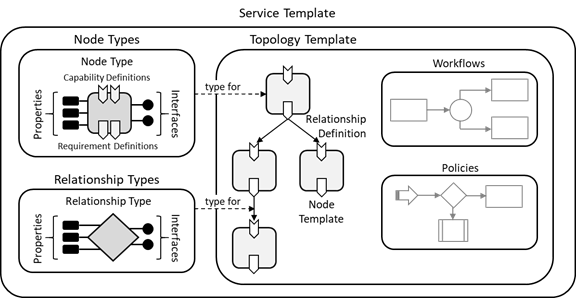
\includegraphics[width=14cm]{tosca_overview}
  \centering
  \caption{Architecture of \gls{toscaacr} and the components of \gls{csaracr} files \cite{tosca_standard_v2}} %TODO add source: official tosca spec
  \label{image:tosca_overview}
\end{figure}

Because the parts (for example a web application on a web server that references a database on another server) can often be reused for other infrastructure parts (or other applications), it makes sense to split a generic description for those parts from the concrete case-specific definition. \Gls{toscaacr} does this with its type definitions. They are optional and not part of the Topology Template, and their sole purpose is to provide a generic template of a component. They can best be described as building blocks, whereas the Topology Template is the actual recipe. It is important to not get confused by the fact that \gls{toscaacr} has three layers of abstraction: The most generic description of a component is the corresponding type. The type defines which properties are allowed, required, what their datatype is and which connections to other components are allowed or required. Derived from this type is a template. As already stated, the template is part of the Topology Template, which describes the actual desired state. The template contains all the information required to instantiate it. 
\newline
The standard allows for different kinds of types; The most important type is the node type. In \gls{toscaacr} context, the term \textquote{node} does not only refer to machines or servers but all components that can be defined via software. This includes low-level applications like operating systems, intermediate middleware programs like web and database servers, as well as high-level software like the web applications running on them. The other types have a more specialized purpose. For example, artifact types are used to describe constant artifacts like \gls{osacr}-images, scripts, and other external (as in non-\gls{toscaacr}) files. The type categories are data-, capability-, interface-, relationship-, group- and policy-types. For most types, there are predefined/default ones, as the basic \gls{yaml} types like string, integer, etc. for datatypes. Custom ones can be added though, as well as composite datatypes. The other types are either self-explaining or not necessary to understand for this thesis. Except for the capability and requirement system, which is worth additional explanation. To reflect where relationships are allowed (for example a web application cannot run on a database server), the standard has the aforementioned system. Corresponding capabilities interlock with requirements like puzzle pieces. An example: Assuming a node has a requirement \textquote{container runtime}, it can only be assigned to an underlying node that offers a capability with the same name. To satisfy this constraint, \gls{toscaacr} orchestrators know they need a node that offers that capability. If there isn't one, they will try to create one. If the container runtime itself has other requirements like \textquote{compute}, the orchestrator will resolve those as well.
Figure \ref{image:tosca_layers_and_requirements} displays how types and templates correspond and how requirements and capabilities are mapped.

\begin{figure}[H]
  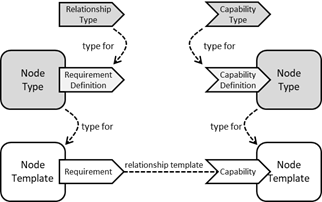
\includegraphics[width=14cm]{tosca_layers_and_requirements}
  \centering
  \caption{Derivation and relationships between \gls{toscaacr} elements \cite{tosca_standard_v2}}
  \label{image:tosca_layers_and_requirements}
\end{figure}

The last part contained in \gls{csaracr} files are management plans. They describe the lifecycle of nodes and how to achieve them. Examples are instantiation, configuration and deallocating/uninstallation/deletion (depending on their type) of nodes \cite{tosca_standard_v2}.
\newline
The standard supports imports with or without namespacing. One common import is the Simple-Profile extension.
It adds a basic set of predefined types to the standard, for example, the node-types Compute, Webserver, and Webapplication with necessary (default) properties, requirements, and capabilities.
\newline
Another important feature of the \gls{toscaacr} standard is \textquote{substitution}. It allows users to outsource the definition of a specific node template to a completely different \gls{csaracr} package. This allows splitting and distribution of concerns and strongly increases the reusability of components. The architecture of the \gls{csaracr} files and the ability of inclusions and substitutions make it also relatively easy to find the corresponding code for a certain component. Figure \ref{image:tosca_substitution} visualizes this substitution approach.

\begin{figure}[H]
  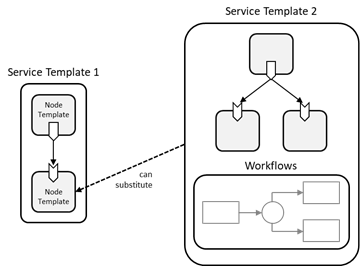
\includegraphics[width=14cm]{tosca_substitution}
  \centering
  \caption{Substitution of node templates with external topologies \cite{tosca_standard_v2}}
  \label{image:tosca_substitution}
\end{figure}

While \gls{toscaacr} does not seem to be very widespread, its origin from OASIS and the many and huge companies backing it and involved in its development make it a very promising standard. The current state of the specification is unfinished, and it is hard to get started in other ways than reading the specification.
\newline
The two most commonly used implementations of \gls{toscaacr} are OpenTOSCA and Cloudify (the latter with its own \gls{toscaacr}-extension). All those preexisting orchestrators have the same approach: They have a web-based frontend, where deployments are managed. In some cases like Cloudify, an additional command-line tool exists, which communicates with the web-based orchestrator via an \gls{apiacr}. The orchestrator is therefore needed to run at all times and needs to have access to the whole infrastructure. The web-based design allows for easy integration with authentication services like LDAP.


% TODO integrate the following findings into this and the previous sections.

% Tosca/cloudify:
%   structure:
%     - how to actually write components and templates is hard to find in the docs -> \url{https://docs.cloudify.co/latest/developer/writing_plugins/creating-your-own-plugin/#writing-plugin-operations}
%     - TOSCA/cloudify standard
%   optimizations:
%     - parallelism, resource graph
%   extensibility:
%     - plugins can be extended, and written by yourself, blueprints
% - see notes.md
% ---
% Tosca/simple-profile:
%   approach:
%     - types, automated type-matching (same name for instances of different types -> tosca automatically matches correct type)
%     - other types:
%       - scalar-unit: <scalar> <unit> % whitespace between is allowed but not required, case-insensitive
%         types:
%         - scalar-unit.size == 1 B, ..., 2 TiB
%         - scalar-unit.time == 1d, 2h, ..., 3ns
%         - scalar-unit.frequency == 1Hz, ..., 5GHz
%         - scalar-unit.bitrate == 1bps, ..., 2GBps, 3TiBps
%       - node-states:
%         - initial: not created, only defined in template
%         - creating -> created
%         - configuring -> configured
%         - starting -> started
%         - stopping -> configured
%         - deleting -> not longer tracked
%         - error
%     - reusable modeling definitions:
%       - description: <string>
%       - metadata: <map>
%       - constraint: [<operators>] % usable on integer, float, timestamp, string, version and scalar-unit % "schema" is special
%       - <property-filter-definition>, f.e. % see structure
%         node_filter:
%           properties:
%             - <something>
%           capabilities: % first checked whether cap is a symbolic name and second if it is a type name
%             - <something>
%       - repository: defined by [ description, url, credential ], but only url is required
%       - <artifact_name>: defined by [ type, file, [deploy_path,checksum,...]] % could contain simple txt-files or disk image with checksum (example in spec at 3.6.7.3)
%       - imports: [uris] % see prefixes and namespaces
%       - <property_name>: [ type, description, required, default, status (supported), constraints, key_schema, entry_schema, external-schema, metadata ]
%       - <attribute_name> [ type, description, default, status, key_schema, entry_schema ]
%       - output_name: [ [SELF|SOURCE|TARGET], attribute_name, ...] % named output
%       - operation implementation, <operation_name>: [ primary (f.e. if primary script in scar file), dependencies (other operations), operation_host ([SELF|HOST|SOURCE|TARGET|ORCHESTRATOR]), timeout] 
%       - operation, <operation_name>: [ description, implementation (<operation implementation>), inputs, outputs ] % execute script or command
%       - (similar to operations) notification, <notification_name>: [ description, implementation, outputs ]
%       - interface: [ inputs, operations, notifications ]
%       % form here onwards, only the typenames are listed
%       - event filter
%       - trigger definition
%       - activity
%       - set state of node by activity
%       - call operation activity
%       - inline workflow
%       - assertion
%       - condition clause (and, or, not, assert)
%       - workflow precondition
%       - workflow step
%       % type-specific definitions:
%       - entity type schema
%       - capability
%       - requirement
%       - artifact
%       - interface type
%       - data type % f.e. phone number
%       - capability type
%       - requirement type
%       - relationship type
%       - group type
%       - policy type
%       % template-specific definitions
%       - capability assignment
%       - requirement assignment
%       % node template
%       % relationship template
%       % group definition
%   hidden-dependencies:
%   structure: % how tosca works https://docs.oasis-open.org/tosca/TOSCA/v2.0/csd03/TOSCA-v2.0-csd03.html#_Toc56506180
%     - my_node_template
%         requirements:
%         - host:
%             node_filter:
%               capabilities:
%               - host:
%                   properties:
%                   - num_cpus: { in_range: [1,4] }
%                   - mem_size: {greater_or_equal: 512MB }
%   validation/error-reporting:
%   aspects to learn:
%     - YAML (since v2)
%     - tosca % there is tosca v1 and v2, but v2 seems to be a copy of v1 so far... but it feels a bit more concise/readable in its structure | v1 == xml, 2v == yaml
%     - tosca simple profile % actually, this is the more important standard, tosca itself is about more abstract stuff
%     - one-time setup of "everything-as-a-service", then only the derived types etc are required to learn
%   tooling/ecosystem:
%     - winery, vinothek -> docker image not working
%     - (cloudify)
%   optimizations:
%     - none?
%   extensibility:
%     - very flexible, as the standard can be extended a lot
%   guarantees:
%     - none?
%   reusability of components:
%     - type definitions can be reused
%     - template definitions can be reused
%     - csar application archive format
%   visibility:
%     - definitions, types, plans, etc feel hard to distinguish
%   viscosity:
%     - definitions have version-fields
%     - updatability seems great so far.
%   consistency:
%     - really great
%   notes:
%     - where does yaml-schema fit in? this seems to define its own meta-schema?
%     - cloudify and alien4cloud used tosca before spec reached final state: https://gitter.im/ystia/yorc?at=5e3b29bfbfe65274eae0f3d0

% \url{https://www.slideshare.net/openstackil/heat-tosca}
% HOT == Heat Orchestration Template, YAML only
% came to replace cloud formation syntax
% following the cloudformation limited model
% hot is only for infrastructure creation
%! tosca is application centric by design
%! -> tosca is more universal
%! hot workflow hardcoded in heat engine
%! toscas interfaces allow for any workflow -> no hardcoded workflow
%! tosca to hot translator project developed by ibm, huawei and others -> goal is to describe stack in tosca and use heat
% cloudify uses tosca templates directly
%   soon to use heat to orchestrate infrastructure
%   adds monitoring, log collection, analytics, workflows

%! tosca adopted hot input and output parameters, which took that from cloudformation
% hot added software\_config provider to describe application stack explicitely
% hot adopted tosca relationship syntax and semantics

% \url{https://www.oasis-open.org/committees/download.php/56826/OpenStack%202015%20Tokyo%20Summit%20-%20TOSCA-and-Heat-Translator-TechTalk.pdf}
% "TOSCA-Parser" by IBM, can parse TOSCA Simple Profile in YAML
% "Heat-Translator", maps and translates non-heat (f.e. tosca) templates to hot
%   supports tosca csar
% "Murano" == OpenStack's application catalog that provides application packaging, deployment and lifecycle management - plans to integrate tosca csar

% \url{https://wiki.openstack.org/wiki/Heat/DSL2}
% evolved first heat/dsl and incorporate tosca and CAMP

% Terraform
% - AWS CloudFormation
%   - \url{https://en.wikipedia.org/wiki/RAML\_(software)} -> supported by aws api
% OpenStack Heat -> can use TOSCA
% Cloudify -> uses TOSCA
% ... (see notes)

% Terraform is very similar to tosca, but because its usability is higher and its learning curve is steeper, its a lot more user friendly.

% %TODO application-distribution -> TOSCA CSAR, helm charts, openstack hot packages in murano...
% - CAMP \url{http://docs.oasis-open.org/camp/camp-spec/v1.1/cs01/camp-spec-v1.1-cs01.pdf} , \url{https://en.wikipedia.org/wiki/Cloud\_Application\_Management\_for\_Platforms}
% - Terraform (describes itself as standard: \url{https://www.terraform.io/intro/vs/custom.html} )
% - cloudformation \url{https://www.terraform.io/intro/vs/cloudformation.html}

\subsection{Selection}
As can be seen, by both the number of initial candidates and the length of the selection process, deciding for a \gls{dslacr} is hard. In this case, it \textquote{only} influences the further course of the thesis, but organizations have the same struggle (based on the number of comparisons and recommendations that circulate the internet). %TODO source
This is due to the nature of these languages: As soon as one is used, it is not feasible to move to another soon. The organization is locked into it. What cross-platform tools and languages like Terraform accomplish is abstracting the vendor lock-in away by language lock-in. Before the rise of \gls{iacacr}, organizations had to go through a similar selection process for their providers. With \gls{iacacr}, organizations now have to select a language that supports all potential providers, has a huge and active user and developer base, so all development on it distributes across many organizations.
\newline
As of 2021, Terraform is the state of the art: It supports more providers than any organization should want to use simultaneously, has the largest market share, and is considered by most providers as a key player \cite{jetbrains_devops_ecosystem_2019}. Therefore, its ecosystem grows and matures exponentially. It has achieved economies of scale and almost a monopoly on cross-provider \gls{iacacr}.
\newline
\Gls{toscaacr} on the other hand is backed by many important companies and is even more customizable than Terraform. Instead of the plugin system, it is based on importable components. While Terraform supports multiple providers in the same infrastructure, moving between providers for the same feature (for example switching the cloud provider) requires manual work. With \gls{toscaacr}s namespacing and substitution system, it is possible to be completely provider-agnostic. At the same time, it does not force (or at least strongly recommend) a new language on its users, as does Terraform with \gls{hclacr}. Additionally, the preexisting types of \gls{toscaacr}s Simple-Profile extension already include types that are necessary for bare metal, for example, the image file type. Another point goes to \gls{toscaacr} because its extensible design makes it possible to include foreign \gls{dslacr}s for their dedicated tasks. An example is that implementations can be written in bash- or python-scripts 
\newline
Because \gls{toscaacr} has a more generic approach and already somewhat aims at working with bare metal, this thesis is going to work with this \gls{dslacr}.

% ---
% there are two types so far:
% - cli, where the dsl is "not perfect" (cloudformation, heat)
%   - hcl vs yaml https://xkcd.com/927/
%     - (?) hcl to json is hard, yaml to json is easy
%     - hcl is optimized for terraform and other hashicorp products
%     - hcl tooling isn't good (even basic linting doesnt exist/work)
% - "perfect dsl" without cli tools and undefined everything as a service (tosca)
% potential main goals:
% - implement cli tool for tosca(-extension) (and design corresponding everything-as-a-service reference definitions)
%   - init command generates definitions
%   - minify removes unused definitions
% - implement tosca parser for terraform/hcl
% additional goals possible:
% - implement one or two reference providers (direct)
% - 
% ---
% implementation details (terraform):
% - grpc as rpc between modules / for plugin-architecture, requires server and clients to be running in parallel - how to start on demand?
%   - ssl/tls by default
%   - grpc-web might enable gui-stuff
% - statefile? namespacing for performance?
% ```
% ------------------------------------------------------------------------------------------------------------------------------------

%TODO how does deprovisioning work
%TODO how are existing resources referenced
%TODO how to handle secrets in outputs
%TODO how to handle secrets in templates
%TODO noecho in cloudformation still shows stuff in output, metadata etc -> how to provide a secure way not giving away credentials?

%TODO -> how can those standards be improved? And what can be added?

% \section{Everything-as-a-Service}
% - can openstack do all of this?
%   - stability
%   - legacy code
%   - complexity
% - Rackspace-as-a-Service; will-on-prem die? ("Why on-prem won't die") no, security of data, costs, privacy, pressure/trust, (with or without pdu, usc, ups)
% - Metal-as-a-Service; vs VM-as-a-Service (vps), noisy neighbour, vSphere AutoDeploy, Ironic, tinkerbell, ipv6, which os, ipmi, kernel/firmware integrity, zones, pdu, psu, rack, sdn
% - Network-as-a-Service; topology, vlan, sdn, both on hw and sw layer
% - DNS-as-a-Service; global or not? via k8s?
% - Hypervisor-as-a-Service; esxi, kvm (used by aws, gcp (no qemu)), node-size, vm-size, compare to metal-as-a-serice (differentiate)
% - Compute-as-a-Service; vm-as-a-service, vps
% - Encryption-as-a-Service: ram, disk, network on host/node-level (TPM?)
% - Storage-as-a-Service; alternative to rook, hyper-converged vs dedicated (SVC by IBM), sds, both on hw and sw layer
% - IAM-as-a-Service; webauthn with yubikey, cloud-iam, 3rd-party iam like github oauth (openstack iam? ad necessary? why no ad join for nodes? -> linux, ephemereal, cattle)
% - k8s-as-a-Service; which os, in-memory-os, cluster-api (gardener, how to configure nodes? Terraform, ansible, cloud-init, ignite), why multi-tenacy via multi-cluster?
% - IaC-as-a-Service; generation/compliance with OPA, CRD-like formal description, check GCP, AWS, Azure and Openstack for common ground
% - secrets-as-a-Service; turtles all the way down presentation, SCM, orchestration, Secrets-as-a-service (hashicorp vault?)
% meta/mgmt
% - bare-metal-marketplace

\section{Reference infrastructure}
% basically: why is os provisioning sufficient



- Are VMs dead? / will containers replace them completely? (/ the case for bare-metal)
  - isolation level
  - comparison of bare-metal approach vs vSphere and/or OpenStack approach
  - constraints like
    - Workload comparison; are there workloads that cannot run in containers and require VMs?
    - minimum machine size defines minimum cluster size and therefore introduces unused resources (when going for temporary k8s-clusters for devs)
  - -> VMs make sense! What about their overhead? They need "zone/node affinity" as well
  - kubevirt?
- common components:
  - public or not (dns / routing)
  - load-balancer / ha
  - persistent or not / storage
  - web-service / api -> should mirror most applications and uses other components
    - db-api
    - web-api
    - REST(ful)-API / CRUD (create, read, update, delete or in HTML: put, get, put, delete, or combine with post)
    - ACID
  - identity / email ?
  - function-as-a-service / serverless -> special case
  - trend:
    - \url{https://en.wikipedia.org/wiki/Resource-oriented_architecture}, \url{https://en.wikipedia.org/wiki/Resource-oriented_computing}, \url{https://en.wikipedia.org/wiki/Service-oriented_architecture}, \url{https://en.wikipedia.org/wiki/Web-oriented_architecture}
    - include example in reference architecture?
    - open data protocol \url{https://en.wikipedia.org/wiki/Open_Data_Protocol}
    - \url{https://en.wikipedia.org/wiki/RSDL}
    - \url{https://en.wikipedia.org/wiki/OpenAPI_Specification} (formerly swagger)
- %TODO where does kubernetes fit in?
- hw-security
  - limit available OS images; optimize those for own hw -> less generic drivers, no overall driver-issues, less to support
  - three installation flavors:
    - install with pxe
    - install with attached iso (via ipmi or hypervisor)
    - preinstalled virtualdisk (only for vms) -> azure
    - ibm supports only attached iso: \url{https://cloud.ibm.com/docs/bare-metal?topic=bare-metal-bm-mount-iso}
  - firmware
    - some hw supports firmware flashing from os level which can result is hardware damage (increasing voltage etc)
    - either on provision or deprovision task update all firmwares to latest official firmware versions (no matter what was installed before - even if it seems to be that already)
      - on deprovisioning makes more sense, it saves time when provisioning new nodes.
    - upgrades can then happen globally (for all "unused" nodes) and used nodes can be migrated by users (or not...)
    - allow to select which firmware version to have flashed
      - latest is default
      - fix them to current latest version after latest was used
  - \url{https://docs.microsoft.com/en-us/azure/baremetal-infrastructure/concepts-baremetal-infrastructure-overview}
    - ? bare metal is ISO 27001, ISO 27017, SOC1 SOC2 compliant
    - RHEL and SLES only
    - ECC vs EDAC (Error Detection And Correction) module; ECC is in hardware, EDAC in software, when both enabled, they can conflicts, with unplanned shutdowns of a server.
    - managed bare metal; up to OS is managed, then the customer is responsible

% \section{Issues with existing standards and frameworks}
% - no comparison of iac dsls
% - not enough effort to integrate with other tools / dsls / clouds (vendor-lock-in seems desired)
% - either no proper standard (vendor-specific) or not enough support for multiple vendors -> everyone reinvents the wheel and wants to establish the own work as industry-standard
- %TODO: propose solution / new approach -> integrate all, search common ground, can tosca solve this?

%TODO market at bottom of iac
